\begin{frame}{} \LARGE
  \begin{center}
      \textbf{Challenges with MPI+X}
  \end{center}
\end{frame}

\begin{frame}[fragile]{The future is MPI+X}
\begin{itemize}
	\item MPI+OpenMP is too often fork-join.
	\item Pthreads scare people; can't be used from Fortran (easily).
	\item TBB and Cilk come from Intel (FYI: TBB now runs on BGQ).
	\item OpenCL is an eye chart and has no abstraction for performance variability.
	\item CUDA is an X for only one type of hardware (ignoring Ocelot).
\end{itemize}
Never confuse portability with portable performance!
\end{frame}

\begin{frame}{Using MPI+OpenMP effectively} \large 
\begin{itemize}
	\item Private data should behave like MPI but with load-store for comm.
	\item Shared data leads to cache reuse but also false sharing.
	\item NUMA is going to eat you alive.  BG is a rare exception.
	\item OpenMP offers little to no solution for NUMA.
	\item If you do everything else right, Amdahl is going to get you.
\end{itemize}
Intranode Amdahl and NUMA are giving OpenMP a bad name;
fully rewritten hybrid codes that exploit affinity behave very different
from MPI codes evolved into MPI+OpenMP codes.
\end{frame}

\begin{frame}{Fork-Join vs. Parallel-Serialize}
  \begin{center}
    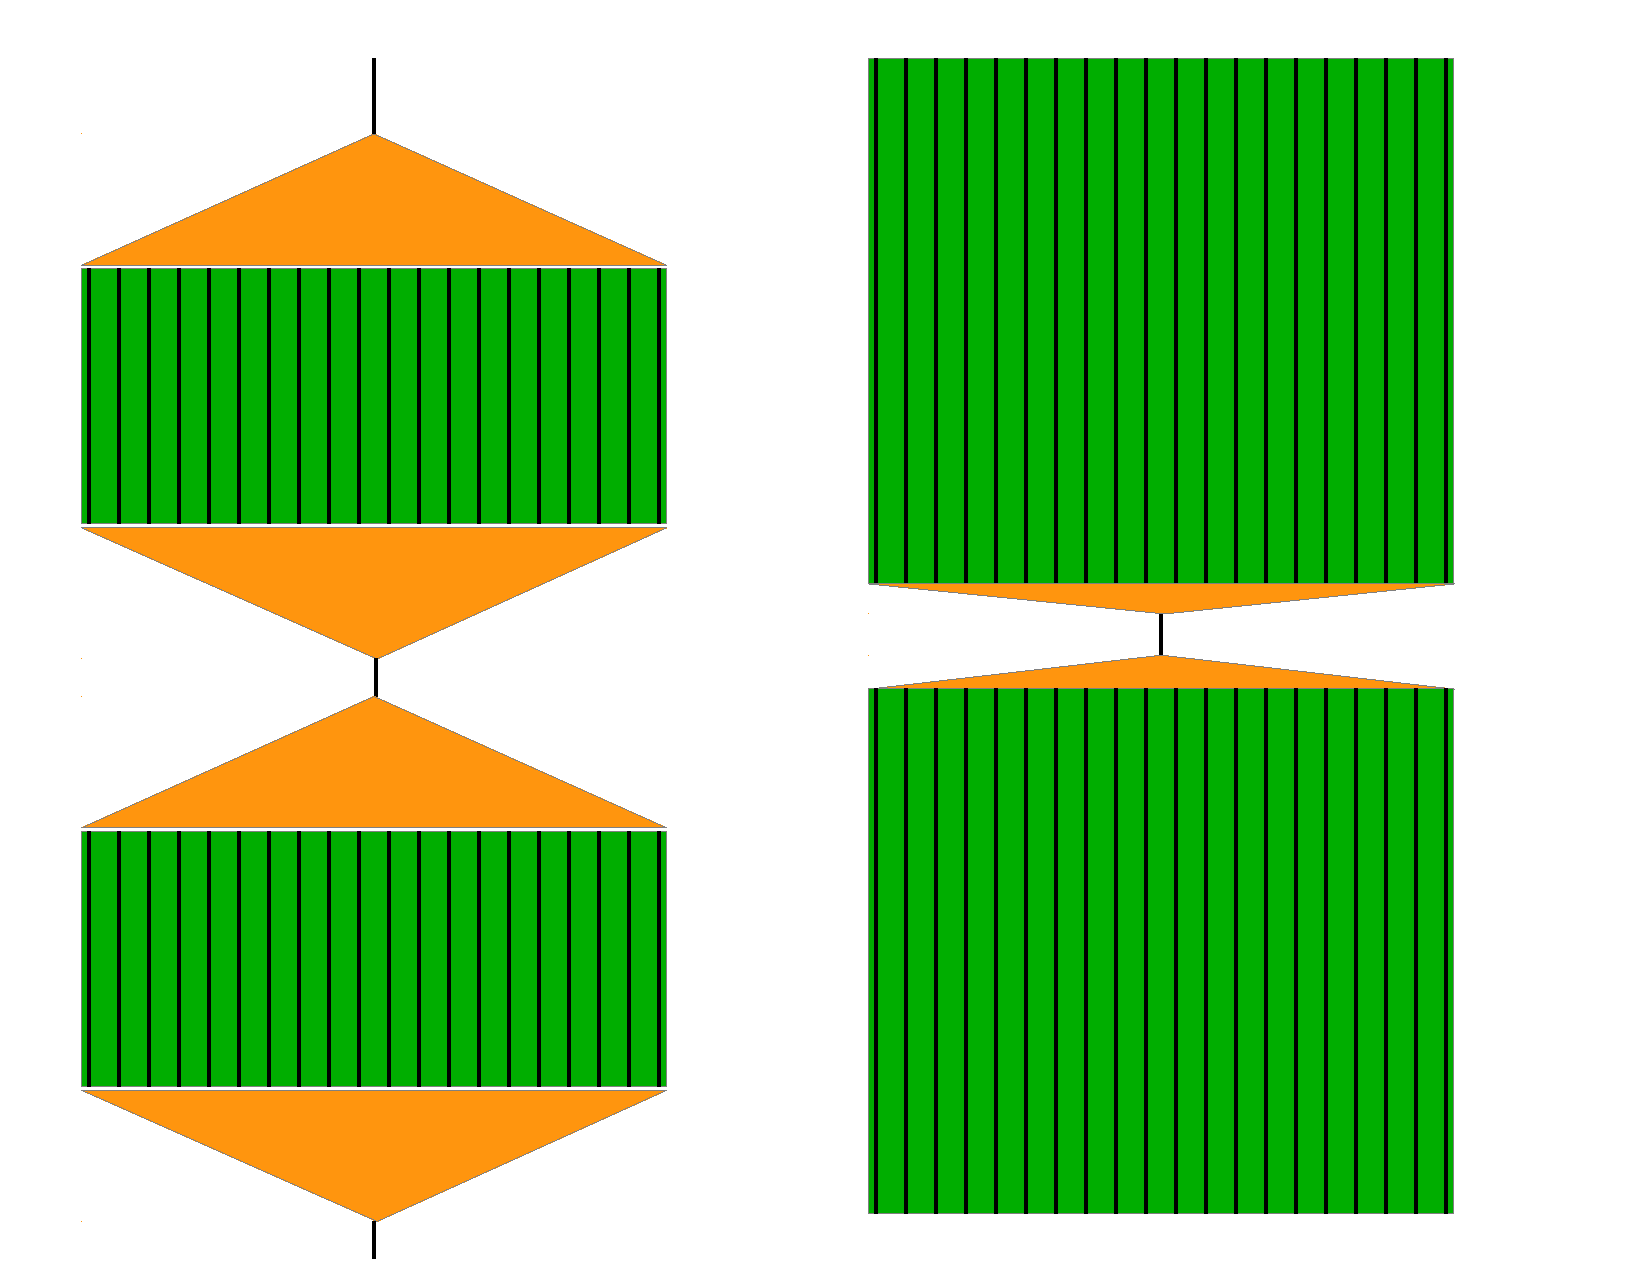
\includegraphics[scale=0.3,angle=0]{ForkJoin.pdf}
  \end{center}
\end{frame}

\begin{frame}{Fork-Join vs. Parallel-Serialize}
  \begin{columns}[T]
    \begin{column}{0.5 \linewidth}
      \begin{tt}
       \color{black}
       \#pragma omp parallel       \\
       \{ \\
       \color{green}
       /* thread-safe */      \\
       \vskip1ex
       \color{black}
       \#pragma omp single         \\
       \color{red}
       /* thread-unsafe */    \\
       \vskip1ex
       \color{black}
       \#pragma omp parallel for   \\
       \color{green}
       /* threaded loops */ \\
       \vskip1ex
       \color{black}
       \#pragma omp sections       \\
       {\color{green}
       /* threaded work */}  \\
       \}     \\
      \end{tt}
    \end{column}
    \begin{column}{0.5 \linewidth}
      \begin{tt}
       {\color{red} /* thread-unsafe */ }  \\
       \vskip1ex
       \color{black}
       \#pragma omp parallel for \\
       \{ \\
       {\color{green} /* threaded loops */} \\
       \} \\
       \vskip1ex
       {\color{red} /* thread-unsafe */ }  \\
       \vskip1ex
       \color{black}
       \#pragma omp parallel for \\
       \{ \\
       {\color{green} /* threaded loops */ } \\
       \} \\
       \vskip1ex
       \color{red}
       /* thread-unsafe work */  \\
      \end{tt}
    \end{column}
  \end{columns}
\end{frame}

\begin{frame}[fragile]{NUMA}
See \texttt{./src/omp/numa.c}
\begin{verbatim}
> for n in 1e6 1e7 1e8 1e9 ; do ./numa.x $n ; done
n = 1000000    a: 0.009927 b: 0.009947 
n = 10000000   a: 0.018938 b: 0.011763 
n = 100000000  a: 0.123872 b: 0.072453 
n = 1000000000 a: 0.915020 b: 0.811122 
\end{verbatim}
The first-order effect requires a multi-socket system so you will not see this on your laptop.
\vskip1ex
For more complicated data access patterns, you may see this even with parallel initialization.  
In this case, consider (1) hiding latency, (2) not being bandwidth bound, and (3) task parallelism.
\end{frame}

\begin{frame}{MPI+Y} \large 
\begin{itemize}
  \item If you use OpenMP libraries built with multiple compilers, you may get multiple thread pools.
  \item OpenMP, TBB, etc. all use Pthreads.  So do many apps and libraries.  Oversubscribe much?
  \item \texttt{MPI\_THREAD\_MULTIPLE} adds overhead; some apps use their own mutex 
  but internal mutexes are invisible to other MPI clients.
\end{itemize}
The stark reality is that general MPI+Y -- i.e. MPI+X for X$\ne$OpenMP -- is heavily dependent
upon an MPI implementation that is designed to be used in a truly multithreaded way.
Today, only Blue Gene/Q as this.
\vskip1ex
{\small Based on \url{https://www.ieeetcsc.org/activities/blog/challenges_for_interoperability_of_runtime_systems_in_scientific_applications} }
\end{frame}



